\documentclass[xcolor={table,usenames,dvipsnames}]{beamer}
\usepackage{eso-pic} 
\usepackage[absolute,overlay]{textpos}
\usepackage{colortbl}
\usepackage{fourier}
\usepackage{booktabs}% http://ctan.org/pkg/booktabs
\newcommand{\tabitem}{~~\llap{\textbullet}~~}
\usepackage{tabularx}
\setbeamertemplate{blocks}[rounded][shadow=true]
\let\olditem\item
\renewcommand{\item}{%
\olditem\vspace{0pt}}     
\usepackage{ragged2e}

%\usepackage[round]{natbib} % incompatible avec biblatex
\usepackage{hyperref}
\hypersetup{
    colorlinks=true,
    linkcolor=.,
    filecolor=deepblue,      
    urlcolor=deepblue,
    pdftitle={Overleaf Example},
    pdfpagemode=FullScreen,
    citecolor=deepblue
    }
\definecolor{LightCyan}{rgb}{0.88,1,1}   
\usepackage[justification=centering]{caption}
\captionsetup{font=scriptsize}
\captionsetup[figure]{name=Fig.}
\captionsetup[table]{name=Tab.}
\setbeamertemplate{caption}[numbered]
\usepackage[T1]{fontenc}
\usepackage{ctex}
\UseRawInputEncoding
%\usepackage[backend=bibtex, style=authoryear, natbib=true, sorting=nty, backref=true]{biblatex}
\usepackage[style=authoryear, maxbibnames=99, mincitenames=1, maxcitenames=2, backref=true, hyperref=true, dashed=false, firstinits=true, backend=bibtex, bibencoding=utf8, uniquename=false, uniquelist=false, natbib=true]{biblatex}
\renewcommand*{\bibfont}{\footnotesize}

% Remove quotation marks from titles
\DeclareFieldFormat[article,incollection,inproceedings,conference]{title}{#1} 
\addbibresource{ref.bib}

%\usepackage[backend=bibtex,
%style=authoryear,
%natbib=true,
%sorting=nty,
%backref=true
%]{biblatex}

\let\oldnocite\nocite
\makeatletter
\renewcommand*{\nocite}[1]{\oldnocite{#1}\Hy@backout{#1}}
\makeatother

\renewcommand*{\bibfont}{\footnotesize}

\DeclareCiteCommand{\cite}
  {\usebibmacro{prenote}}
  {\usebibmacro{citeindex}%
   \printtext[bibhyperref]{\usebibmacro{cite}}}
  {\multicitedelim}
  {\usebibmacro{postnote}}

\DeclareCiteCommand*{\cite}
  {\usebibmacro{prenote}}
  {\usebibmacro{citeindex}%
   \printtext[bibhyperref]{\usebibmacro{citeyear}}}
  {\multicitedelim}
  {\usebibmacro{postnote}}

\DeclareCiteCommand{\parencite}[\mkbibparens]
  {\usebibmacro{prenote}}
  {\usebibmacro{citeindex}%
    \printtext[bibhyperref]{\usebibmacro{cite}}}
  {\multicitedelim}
  {\usebibmacro{postnote}}

\DeclareCiteCommand*{\parencite}[\mkbibparens]
  {\usebibmacro{prenote}}
  {\usebibmacro{citeindex}%
    \printtext[bibhyperref]{\usebibmacro{citeyear}}}
  {\multicitedelim}
  {\usebibmacro{postnote}}

\DeclareCiteCommand{\footcite}[\mkbibfootnote]
  {\usebibmacro{prenote}}
  {\usebibmacro{citeindex}%
  \printtext[bibhyperref]{ \usebibmacro{cite}}}
  {\multicitedelim}
  {\usebibmacro{postnote}}

\DeclareCiteCommand{\footcitetext}[\mkbibfootnotetext]
  {\usebibmacro{prenote}}
  {\usebibmacro{citeindex}%
   \printtext[bibhyperref]{\usebibmacro{cite}}}
  {\multicitedelim}
  {\usebibmacro{postnote}}

%\DeclareCiteCommand{\textcite}
%  {\boolfalse{cbx:parens}}
%  {\usebibmacro{citeindex}%
%   \printtext[bibhyperref]{\usebibmacro{textcite}}}
%  {\ifbool{cbx:parens}
%     {\bibcloseparen\global\boolfalse{cbx:parens}}
%     {}%
%   \multicitedelim}
%  {\usebibmacro{textcite:postnote}}

        \DeclareCiteCommand{\textcite}
        {\usebibmacro{cite:init}%
            \usebibmacro{prenote}}
        {\usebibmacro{citeindex}%
            \printtext[bibhyperref]{\usebibmacro{textcite}}}
        {}
        {\printtext[bibhyperref]{\usebibmacro{textcite:postnote}}%
            \usebibmacro{cite:post}}

\addbibresource{ref.bib}

% Cannot enable in Xelatex
\usepackage{pgfpages}
% \setbeameroption{hide notes} % Only slides
% \setbeameroption{show only notes} % Only notes
% \setbeameroption{show notes on second screen}

% other packages
\usepackage{latexsym,amsmath,multicol,booktabs,calligra}
\usepackage{graphicx,listings,stackengine}
\usepackage[greek,french]{babel}
\usepackage[LGR,T1]{fontenc}
\usepackage{fontspec}

%\usepackage[sfdefault,light,scaled=.85]{merriweather} %% Option 'black' gives heavier bold face 


\usepackage[sfdefault]{AlegreyaSans} %% Option 'black' gives heavier bold face
%% The 'sfdefault' option to make the base font sans serif
\renewcommand*\oldstylenums[1]{{\AlegreyaSansOsF #1}}



% Define a command for text in Greek. Replace 'Gentium Plus' with a font of your choice if necessary.
\newfontfamily\greekfont{Gentium Plus}
\newcommand{\textgreek}[1]{{\greekfont #1}}

\DefineBibliographyStrings{french}{%
  backrefpage = {voir p\adddot},%
  backrefpages = {voir pp\adddot}%
}
\DeclareFieldFormat{pagerefformat}{\mkbibparens{{\color{red}\mkbibemph{#1}}}}
\renewbibmacro*{pageref}{%
  \iflistundef{pageref}
    {}
    {\printtext[pagerefformat]{%
       \ifnumgreater{\value{pageref}}{1}
         {\bibstring{backrefpages}\ppspace}
         {\bibstring{backrefpage}\ppspace}%
       \printlist[pageref][-\value{listtotal}]{pageref}}}}
\usepackage{wasysym}
% Enable only in Xelatex
 \usepackage{pstricks}

\author[Ljudmila PETKOVIC]{\small \textbf{Ljudmila PETKOVIC}\textsuperscript{1,2,3}\\\medskip{\footnotesize\texttt{prenom.nom@sorbonne-universite.fr}}}
\title[Mesurer l’influence de Jean-Martin Charcot sur ses contemporains$\dots$]{\fontsize{13pt}{13pt}\selectfont Mesurer l’influence de Jean-Martin Charcot sur ses contemporains à l’aide de l’extraction des phrases-clés}
%\subtitle{Approche \textit{PatternRank}}
\institute [JE \og{}Humanités numériques\fg{}] {\tiny \textsuperscript{1} Sorbonne Université, Faculté des Lettres, \textsc{UFR} Littératures françaises et comparée, ED 3\\\textsuperscript{2} Centre d'étude de la langue et des littératures françaises (\textsc{CELLF}), \textsc{UMR 8599}\\\textsuperscript{3} Observatoire des textes, des idées et des corpus (\textsc{ObTIC})}
\date[\textsc{BnF}, le 3 mai 2024]{\scriptsize  Journée \og{}IA et Humanités Numériques\fg{}\\\textsc{BnF}, salle 70\\Paris, le 3 mai 2024}
\usepackage{YTU}

% defs
\def\cmd#1{\texttt{\color{red}\footnotesize $\backslash$#1}}
\def\env#1{\texttt{\color{blue}\footnotesize #1}}
\definecolor{deepblue}{rgb}{0,0,0.5}
\definecolor{deepred}{rgb}{0.6,0,0}
\definecolor{deepgreen}{rgb}{0,0.5,0}
\definecolor{halfgray}{gray}{0.55}
\definecolor{warmblack}{rgb}{0.0, 0.26, 0.26}

\lstset{
    basicstyle=\ttfamily\small,
    keywordstyle=\bfseries\color{deepblue},
    emphstyle=\ttfamily\color{deepred},    % Custom highlighting style
    stringstyle=\color{deepgreen},
    numbers=left,
    numberstyle=\small\color{halfgray},
    rulesepcolor=\color{red!20!green!20!blue!20},
    frame=shadowbox,
}
% \logo{%
%     
\includegraphics[width=1cm,height=1cm,keepaspectratio]{pic/obtic.jpg}~%
%     
\includegraphics[width=1cm,height=1cm,keepaspectratio]{pic/Lettres_su_logo.png}~%
% }
\usepackage{enumerate}
\setbeamertemplate{section in toc}{\hspace*{1em}\inserttocsectionnumber.~\inserttocsection\par}
\setbeamertemplate{subsection in toc}{\hspace*{2em}\inserttocsectionnumber.\inserttocsubsectionnumber.~\inserttocsubsection\par}
\renewcommand*{\bibfont}{\scriptsize}



\let\oldfootnotesize\footnotesize
\renewcommand*{\footnotesize}{\oldfootnotesize\scriptsize}

%\setbeamertemplate{itemize/enumerate body begin}{\small}
\setbeamertemplate{itemize/enumerate subbody begin}{\small}
%
%\newcommand{\leftquote}{{\fontfamily{lmr}\selectfont\textquotedblleft}}
%\newcommand{\rightquote}{{\fontfamily{lmr}\selectfont\textquotedblright}}
%\newcommand{\leftguillemet}{{\fontfamily{lmr}\selectfont\guillemotleft}}
%\newcommand{\rightguillemet}{{\fontfamily{lmr}\selectfont\guillemotright}}







\begin{document}

\begin{frame}
    \titlepage
\begin{figure}
    \centering
    
    
\includegraphics[width=2cm,height=1cm,keepaspectratio]{pic/Lettres_su_logo.png}~\hspace*{0.5cm}%\includegraphics{}
    
\includegraphics[width=2cm,height=1cm,keepaspectratio]{pic/cellf.png}~\hspace*{0.5cm}%
    
\includegraphics[width=3cm,height=1cm,keepaspectratio]{pic/obtic.jpg}~%

\end{figure}
    
    \begin{note}
        {Introduce your self}
    \end{note}

\end{frame}

\begin{frame}
\frametitle{Plan}
    \tableofcontents[sectionstyle=show,subsectionstyle=show/shaded/hide,subsubsectionstyle=show/shaded/hide]
\end{frame}

\section[Contexte]{Contexte de recherche}
%\begin{frame}{Le progrès de la science comme un processus discontinu}
\begin{block}{Rupture épistémologique}
\justifying
Passage radical d'un paradigme\footnote{découverte scientifique universellement reconnue.} à un autre, dans la façon dont les scientifiques abordent un domaine donné.
\end{block}
\begin{itemize}
\small
\item \og{}rupture entre observation et expérimentation \fg{}
{\footnotesize(\cite{bachelard1934formation})}
\item \og{}révolution scientifique\fg{} {\footnotesize(\cite{koyre1957closed})}
\item \og{}changement de paradigme\fg{} {\footnotesize(\cite{kuhn1962structure})} 
\end{itemize} 
%Le nouveau paradigme est incompatible avec le précédent, p. ex. géo- \textit{vs.} héliocentrisme.
\begin{minipage}{5cm}
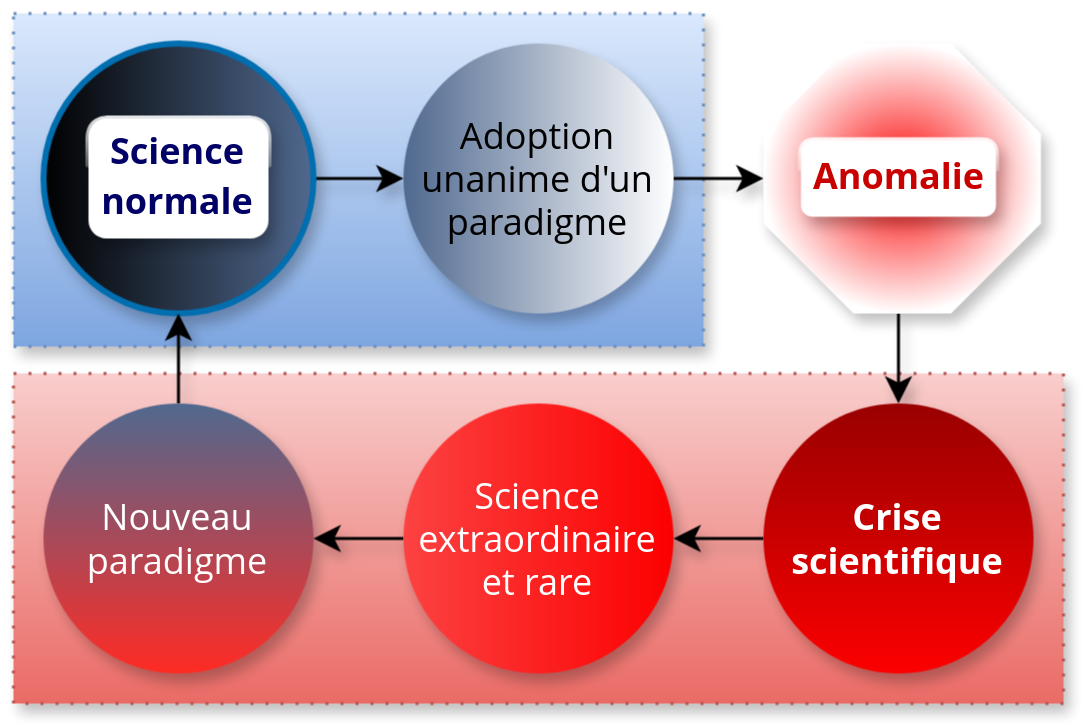
\includegraphics[height=3cm, width=4.5cm]{pic/changement_paradigme.png}
\end{minipage}%
\begin{minipage}{6cm}
{\normaltext Conception kuhnienne du progrès scientifique, adaptée de {\small\textcite{amiri}}}. \bigskip

 {\scriptsize Le nouveau paradigme est incompatible avec le précédent, p. ex. géo- \textit{vs.} héliocentrisme.}
\end{minipage}
%\begin{figure}
%    \centering
%    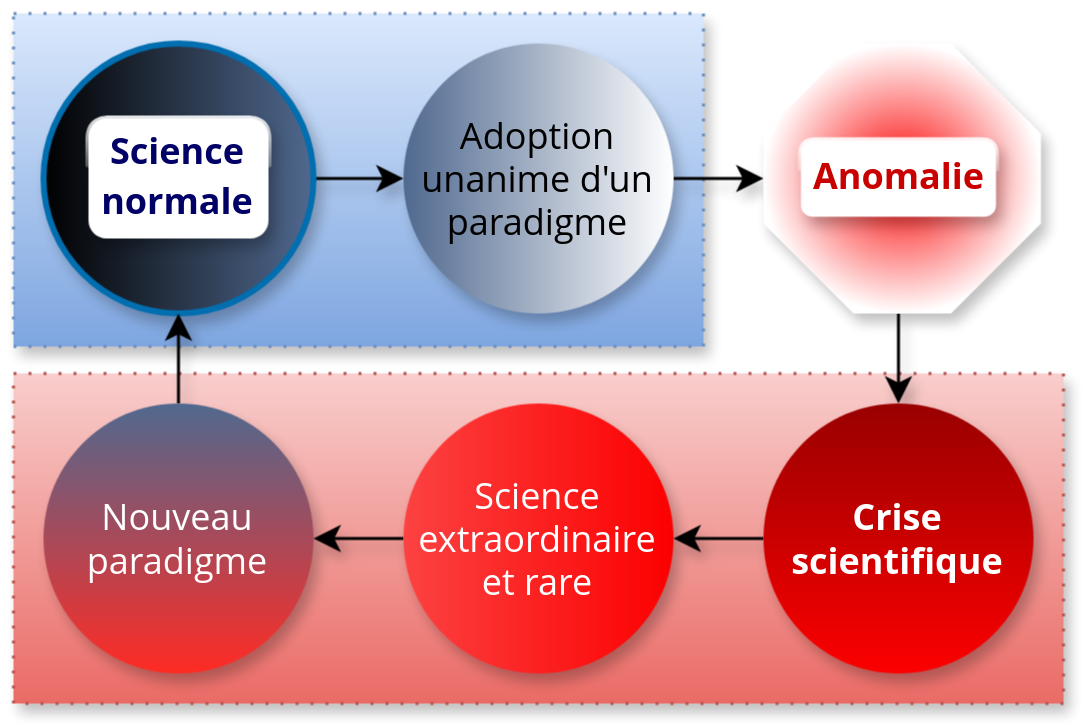
\includegraphics[width=65mm,scale=0.5]{pic/changement_paradigme.png}
%    \caption{Conception kuhnienne du progrès scientifique, adaptée de {\scriptsize\textcite{amiri}}.}
%    \label{fig:enter-label}
%\end{figure}
\end{frame}

%\begin{frame}{Évolution du terme \textit{hystérie}}
Exemple du changement de paradigme : le terme d'\textsc{hystérie}
\begin{itemize}
 \item gr. \textgreek{ὑστέρα}, lat. \textit{hystera} : \og{}utérus\fg{}, \og{}matrice\fg{}
\end{itemize}
\begin{table}[h!]
\footnotesize
\begin{tabular}{lcl}
\multicolumn{1}{l}{\textrm{Période}} & \multicolumn{1}{c}{\textrm{Sexe}} & \multicolumn{1}{c}{\textrm{Étiologie}}   \\
\hline \hline
Antiquité   & \female{}             & \begin{tabular}[c]{@{}l@{}}{\footnotesize déplacement de l'utérus, selon Hippocrate \citep{tasca2012women}
%\footnote{{\footnotesize\cite{tasca2012women}}}
\\\textit{hystérique} : (femme) malade de l'utérus}\end{tabular}          \\ \hline
Moyen Âge   & \female{}             & \begin{tabular}[c]{@{}l@{}}{\footnotesize possession démoniaque, superstition religieuse de l'Église
%\footnote{{\footnotesize\cite{tasca2012women}}}
\\ 	$\rightarrow$ chasses, tortures, exorcismes \citep{tasca2012women}}\end{tabular} \\ \hline
Renaissance & \female{}/\male{}           & \begin{tabular}[c]{@{}l@{}}{\footnotesize localisation dans le cerveau, \textit{sensorium commune} \citep{lepois1618}
%\footnote{{\footnotesize\cite{lepois1618}}}
\\\og{}siège commun de la sensibilité\fg{}\footnote{\cite{kant1863}.}, ensemble des perceptions}\end{tabular}   \\ \hline
Lumières    & \female{}/\male{}           & \begin{tabular}[c]{@{}l@{}}{\footnotesize explosion des \og{}esprits animaux\fg{} dans le cerveau\\maladie convulsive \citep{willispathologiae}\footnote{{\footnotesize créateur du terme \textit{neurologia} en 1664.}}}\end{tabular} \\ \hline
\rowcolor{LightCyan}
\textsc{XIX}\ieme{} s. & \female{}/\male{} & \begin{tabular}[c]{@{}l@{}}{\footnotesize dégénérescence héréditaire du système nerveux \citep{charcot1870}
%\footnote{{\footnotesize\cite{charcot1870}}}
\\maladie systématiquement traitée comme un trouble neurologique}
\end{tabular}
\end{tabular}
\end{table}
\begin{itemize}
\end{itemize}
\end{frame}




\begin{frame}{\og{}Napoléon des névroses\fg{} ou \og{}Paganini de l'hystérie\fg{} {\small(\hypersetup{citecolor=yellow}\cite{marmion2015freud})}}

\textsc{\textcolor{deepblue}{\textbf{Jean-Martin CHARCOT}} (1825-1893)}
%\hbox{\hspace{25em} 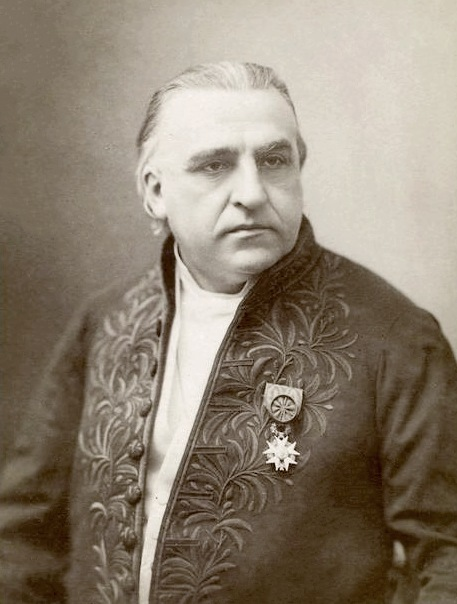
\includegraphics[scale=0.07]{pic/Jean-Martin_Charcot.jpg}}
%\\{\scriptsize Portrait de\\Charcot (\href{https://fr.wikipedia.org/wiki/Jean-Martin_Charcot}{Wikipedia}).}
\hbox{\hspace{10.3em} 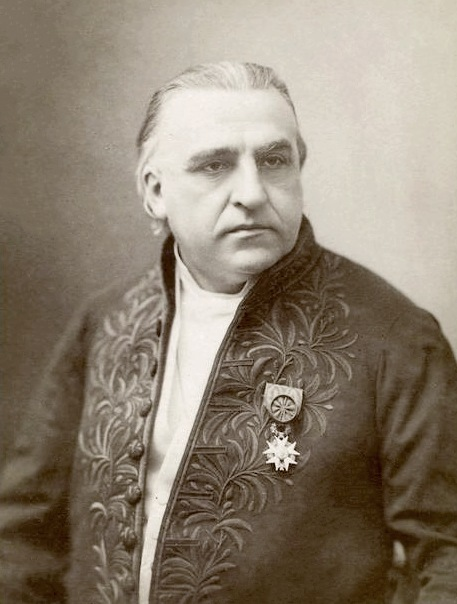
\includegraphics[scale=0.06]{pic/Jean-Martin_Charcot.jpg}}\\\hbox{\hspace{23.8em}{\tiny Source : \href{https://fr.wikipedia.org/wiki/Jean-Martin_Charcot}{Wikipedia}}.}
\begin{itemize}
\item père de la neurologie moderne en France au XIX\ieme{} s. 
\item leçons cliniques du mardi à l'hôpital de la Salpêtrière à Paris \\
\hspace{165pt}
\footnotesize\og{}Mecque de la neurologie\fg{}
\end{itemize}
\begin{enumerate}[\indent {}]
\item Contributions majeures :
\begin{table}[h!]
\small
\begin{tabular}{l l}
\textcolor{darkgray}{hystérie} & $\leftarrow$ lésion dynamique des circuits cérébraux\\
\textcolor{darkgray}{hypnose} & analyse et traitement des symptômes hystériques\\
\textcolor{darkgray}{SEP} & description de la \textit{sclérose en plaques} disséminée\footnote{ou \textit{sclérose multiple}.}\\
\textcolor{darkgray}{SLA} & description de la \textit{sclérose latérale amyotrophique\footnote{\textit{maladie de Charcot} ou \textit{maladie Lou-Gehrig}.}}\\
\textcolor{darkgray}{maladie de Parkinson} & concepteur du terme (avec Alfred Vulpian)
\end{tabular}
\end{table}
%	\begin{description}
%	    \item[hystérie] 
%	    résultat d'une lésion dynamique des circuits cérébraux
%    \item[hypnose] 
%    analyse des symptômes hystériques et outil thérapeutique
%    \item[SEP]\footnote{abbr. \textit{sclérose en plaques}.}
%     disséminée (description) $\rightarrow$ sclérose multiple
%    \item[SLA]\footnote{abbr. \textit{sclérose latérale amyotrophique}.}
%     (description) $\rightarrow$ maladie de Charcot / Lou Gehrig
%    \item[maladie de Parkinson]
%    concepteur du terme (avec A. Vulpian)
%	\end{description}  
	\end{enumerate}
    % \item hystérie est due à une \textit{lésion dynamique} de l’encéphale, liée à un traumatisme de nature physique (accident de train, chute, choc$\dots$) -- possible de recréer sous hypnose
    % \item impact sur les acteurs dans ou en dehors de sa discipline : S. Freud, G. de la Tourette, E. Zola$\dots$
    \begin{flushright}
{\footnotesize(\cite{camargo2024jean})}
\end{flushright}

%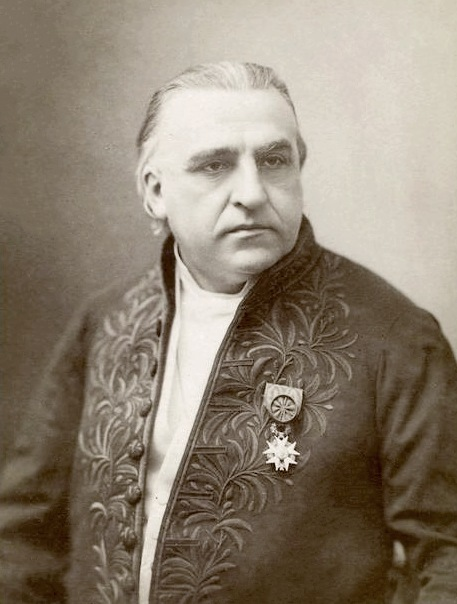
\includegraphics[width=10pt]{pic/Jean-Martin_Charcot.jpg}%
%\\{\scriptsize Portrait de\\Charcot (\href{https://fr.wikipedia.org/wiki/Jean-Martin_Charcot}{Wikipedia}).}



\end{frame}

\begin{frame}{Impact de Charcot sur sa discipline et au-delà}
\centering
\textbf{(Quelques) collaborateurs et élèves}\\
{\small \og{}réseau scientifique\fg{}}
    \begin{table}[!ht]
        \centering
        \small
        \begin{tabular}{l r}
           Sigmund \textsc{Freud} (1856-1939)  & théorie psychanalytique \\
            Gilles \textsc{de la Tourette} (1857-1932) & syndrôme de Tourette \\
            Joseph \textsc{Babinski} (1857-1904) & pithiatisme, signe de Babinski \\
%           Pierre \textsc{Janet} (1859-1947) & psychopathologie
%            dissociation, sous-conscient 
        \end{tabular}
        \begin{flushright}
%        \footnotesize\citep{bogousslavsky2020}
        \footnotesize\citep{BROUSSOLLE2012301}
        \end{flushright}
        % \caption{Caption}
        \label{tab:my_label}
    \end{table}
\medskip
\textbf{(Quelques) écrivains naturalistes français et européens} 
\begin{itemize}
\centering
\small \item références à Charcot et aux descriptions de crises hystériques
\end{itemize}
\begin{table}[!ht]
    \centering
    \small
    \begin{tabular}{l r}
        Émile \textsc{Zola} (1840–1902)  & \textit{Lourdes} \\
        Léon \textsc{Tolstoï} (1828–1910) & \textit{La Sonate à Kreutzer} \\
        Luigi \textsc{Capuana} (1839–1915) & \textit{La Torture}
%        Bjørnstjerne \textsc{Bjørnson} (1832–1910) & \textit{Over Ævne}
    \end{tabular}
            \begin{flushright}
        \footnotesize\citep{koehler2013charcot}
        \end{flushright}
    % \caption{Caption}
    \label{tab:my_label}
\end{table}

\end{frame}



\section[Objectif]{Problématique et objectif}
\begin{frame}{Circulation du discours médical au prisme du numérique}
\centering
Objectif : aborder computationnellement la question des circulations des phénomènes textuels complexes.
\begin{figure}
    \centering
    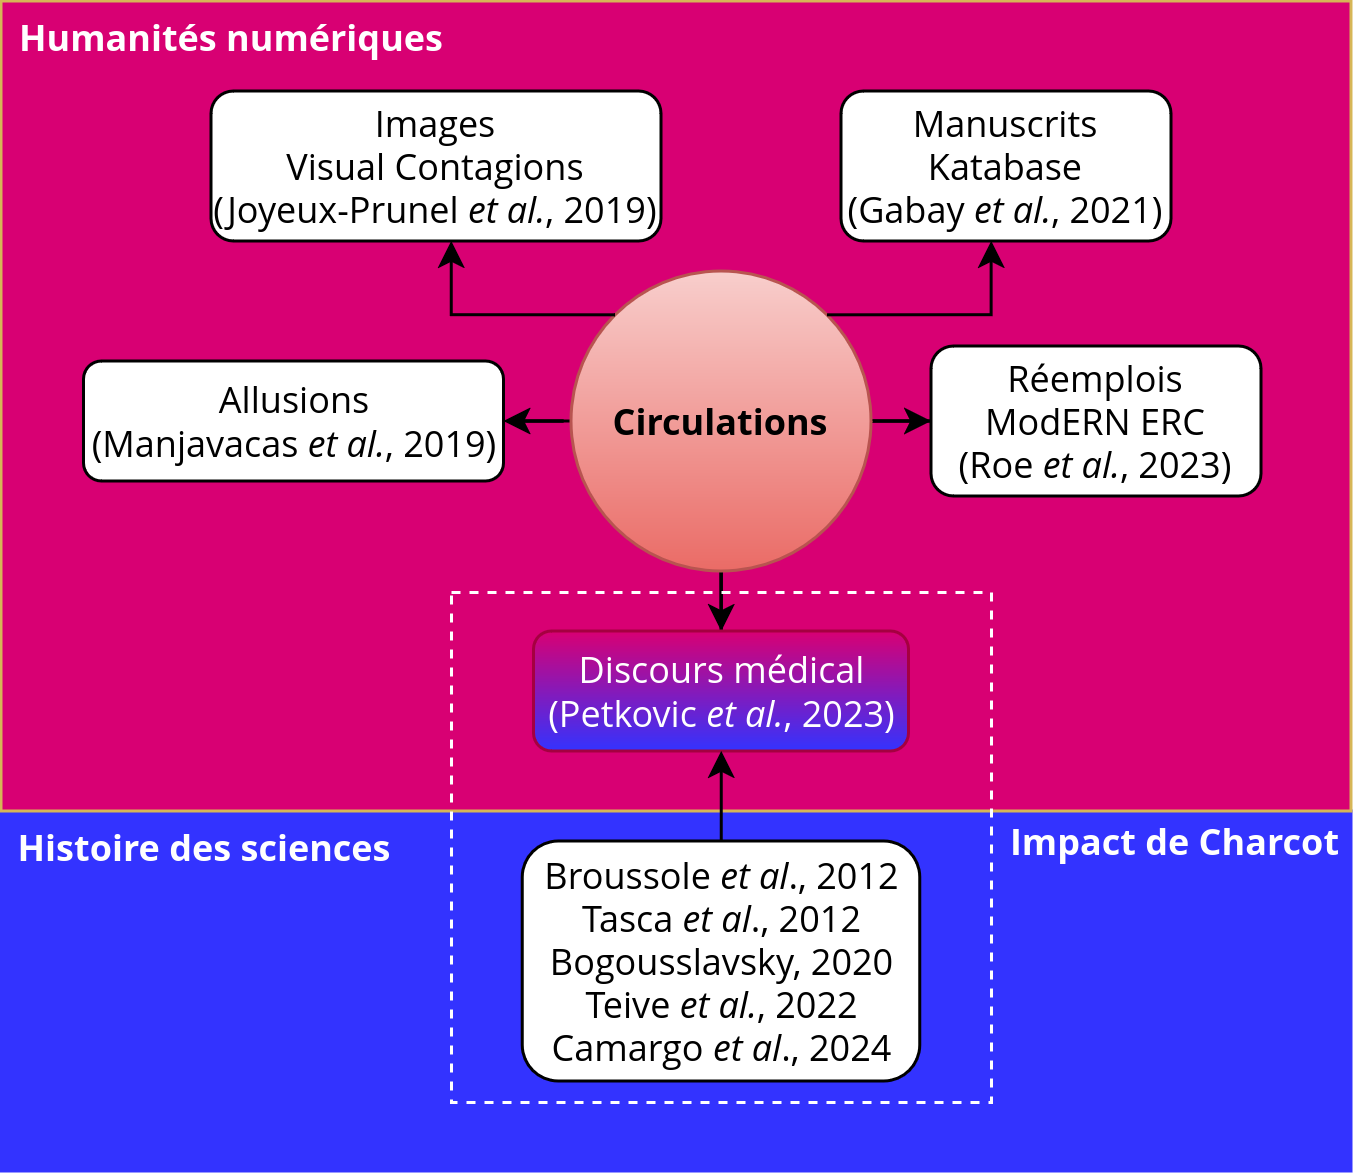
\includegraphics[width=65mm,scale=0.5]{pic/dh_histoire-sciences.png}
    \caption{Études (numériques) des circulations des savoirs.}
    \label{fig:enter-label}
\end{figure}
\notecite{joyeux2019visual}
\notecite{gabay2021katabase}
\notecite{manjavacas2019}
\notecite{tasca2012women}
\notecite{bogousslavsky2020}
\notecite{teive2022thomas}
\nocite{camargo2024}
% Influence de Charcot : \cite{bogousslavsky}, \cite{camargo}
% Constitution et exploitation de ce fonds au prisme du numérique
\end{frame}


\begin{frame}{Question de recherche}
% Comment mesurer le degré d'intertextualité entre Charcot et son réseau scientifique et artistique au prisme du numérique ?
% create the main block
\begin{exampleblock}{}
\centering
    \color{deepblue}{\textmd{Comment mesurer le degré d'intertextualité entre le discours de Charcot et celui de son réseau scientifique au prisme du numérique ?}}
\end{exampleblock}

\end{frame}


\section[Approche supervisée]{Approche supervisée}
\begin{frame}{Fonds Charcot \href{https://patrimoine.sorbonne-universite.fr/collection/Fonds-Charcot}{\textcolor{yellow}{en ligne}}}
\begin{block}{SorbonNum\\
\footnotesize{Bibliothèque de Sorbonne Université (\textsc{BSU})}}
201 documents XML OCRisés (sans post-correction)
\end{block}
%\begin{itemize}
%    \item \textrm{Charcot} : textes rédigés par Charcot
%    \item \textrm{Autres} : textes rédigés par les membres de son réseau scientifique
%\end{itemize}
\begin{table}[!ht]
    \centering
    \begin{tabular}{|c|r|r|}
    \hline 
    \rowcolor{yellow!30}
       Corpus & \multicolumn{1}{c|}{Nb de docs} & \multicolumn{1}{c|}{Nb de tokens} \\
       \hline
      \begin{tabular}[c]{@{}c@{}}\textrm{Charcot}\\ \scriptsize{textes rédigés par Charcot}\end{tabular}  & 68 & 12 190 649 (38,12\%) \\
       \hline
       \begin{tabular}[c]{@{}c@{}}\textrm{Autres}\\ \scriptsize{textes rédigés par les membres} \vspace{-0.15cm} \\ \scriptsize{de son réseau scientifique}\end{tabular}    & 133 & 19 788 830 (61,88\%) \\
       \hline\hline
       \textbf{Total} & \textbf{201} & \textbf{31 979 479} (100\%)\\
       \hline
    \end{tabular}
    \caption{Répartition du fonds Charcot selon les auteurs.
%    \footnote{\tiny{\url{https://patrimoine.sorbonne-universite.fr/collection/Fonds-Charcot}}}
}
    \label{tab:my_label}
\end{table}
\end{frame}

\begin{frame}{Corpus Charcot \href{https://obtic.huma-num.fr/obvie/charcot/?view=corpus}{\textcolor{yellow}{en ligne}}}
Corpus Charcot accessible sur la plateforme \textsc{OBVIE} \hfill {\small\citep{alrahabi2022obvie}}
\begin{itemize}
\item fouille avancée des corpus en \textsc{XML-TEI}
\item textes similaires : mots fréquents / en commun, noms cités
\end{itemize}
%\danger impossible de quantifier l'importance des MWEs
\begin{figure}[!h]
    \centering
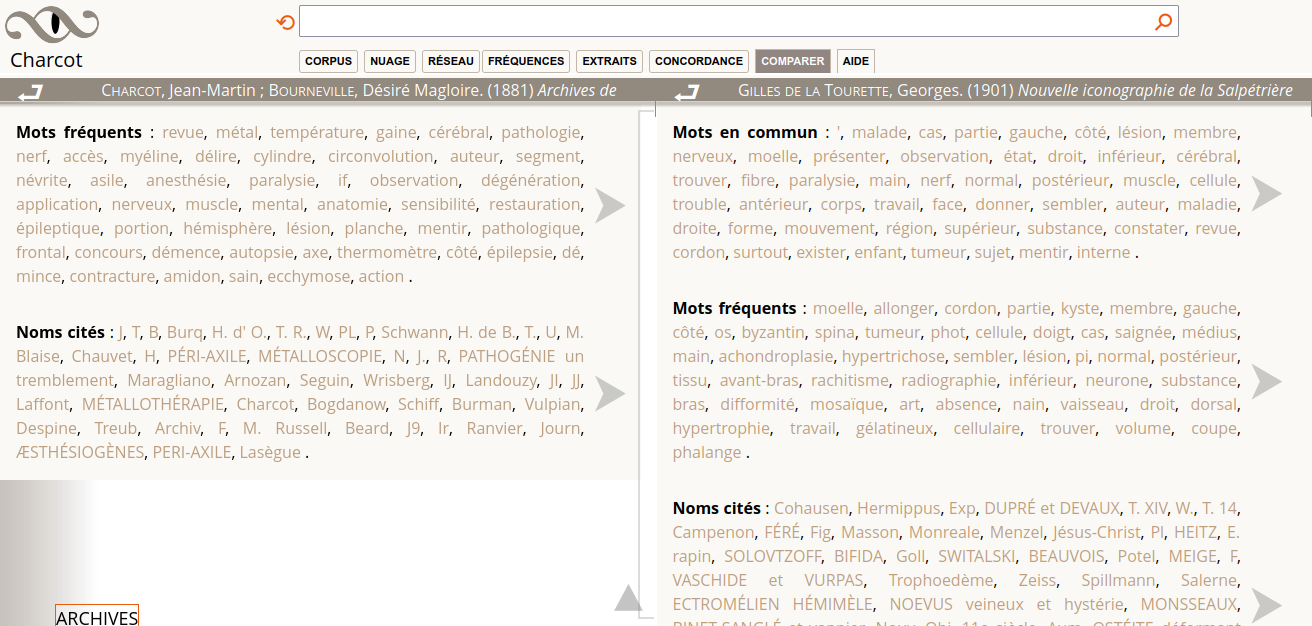
\includegraphics[width=90mm,scale=0.5]{pic/doc_sim.png}
    \caption{Points similaires entre un ouvrage de Charcot et celui de de la Tourette.}
%    \caption{Distribution des fréquences des tokens avec la frise chronologique pour ceux constituant l'expression \textit{bulbe rachidien} (issus des corpus \og{}Charcot\fg{} et \og{}Autres\fg{}).}
    \label{fig:my_label}
\end{figure}
% citations directes (\cite{manjavacas2019})
\end{frame}

\begin{frame}{Mesurer le degré d'intertextualité}
Mesurer informatiquement l'impact de Charcot sur son réseau \\$\rightarrow$ intertextualité uni-directionnelle
\begin{figure}[!h]
    \centering
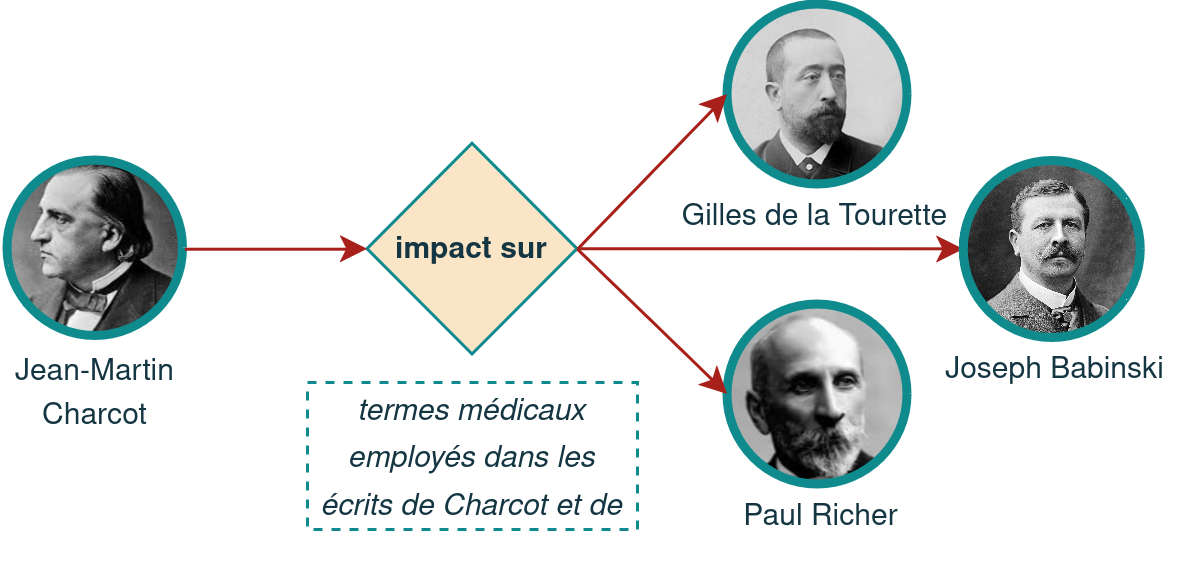
\includegraphics[width=100mm,scale=0.5]{pic/charcot_intertextualite.png}
    \caption{Opérationnalisation de l'impact de Charcot sur ses élèves.}
    \label{fig:my_label}
\end{figure}
\end{frame}

%\begin{frame}{Première analyse}
%\textbf{OBVIE}\footnote{\url{https://obtic.huma-num.fr/obvie/}}
%\begin{itemize}
%    \item moteur de recherche permettant la fouille avancée des corpus en \textsc{XML-TEI}
%    \item identification des substantifs les plus importants de chaque corpus 
%    \begin{itemize}
%        \item fréquences brutes, mesures \textsc{TF-IDF}, \textsc{BM25}, $\chi^2$, Test Gamma
%    \end{itemize}
%    \item repérage des textes similaires par ordre de pertinence à partir des termes en commun
%\end{itemize}
    
%\end{frame}


%\begin{frame}{Deuxième analyse}
%    \textbf{TextPair}\footnote{\url{https://artfl-project.uchicago.edu/text-pair}}
%    \begin{itemize}
%        \item alignement des séquences similaires dans les deux corpus
%        \item génère une liste de passages similaires pour chaque texte
%        \item séquences de mots qui se chevauchent (trigrammes de mots)
%        \item comparer ces résultats avec ceux de séquences dans d’autres textes
%    \end{itemize}
%\end{frame}
%
%\begin{frame}{Deuxième analyse -- TextPair\footnote{\url{https://anomander.uchicago.edu/text-pair/charcot2autres/}}}
%\danger nombre de
%résultats assez conséquent -- filtrage nécessaire
%    \begin{figure}[!ht]
%        \centering
%        \includegraphics[width=90mm,scale=0.5]{pic/textpair.png}
%        \caption{Alignement et comparaison des textes de
%Charcot à celui de Georges Gilles de la Tourette (le seul
%résultat) en lançant la requête \textit{sclérose latérale
%amyotrophique}.}
%        \label{fig:enter-label}
%    \end{figure}
% \end{frame}

\begin{frame}{Liste des concepts médicaux}
Extraction semi-automatique des termes en lien avec Charcot.\\~\\

 \begin{figure}[!htb]
    \centering
    \begin{minipage}{.5\textwidth}
        \centering
        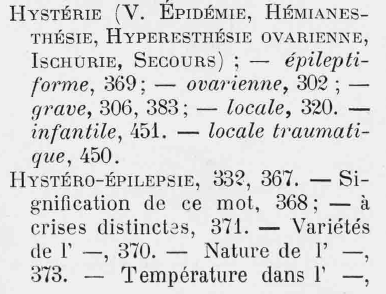
\includegraphics[width=0.6\linewidth, height=0.3\textheight]{pic/concepts-pdf}
        \caption{Index des termes \citep{charcot1890oeuvres}.}
        \label{fig:prob1_6_2}
    \end{minipage}%
    \begin{minipage}{.5\textwidth}
        \centering
        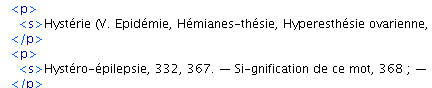
\includegraphics[width=1\linewidth, height=0.15\textheight]{pic/concepts-xml}
        \caption{Concepts médicaux, document XML.}
        \label{fig:prob1_6_1}
    \end{minipage}
\end{figure}
%\begin{figure}[!h]
%    \centering
%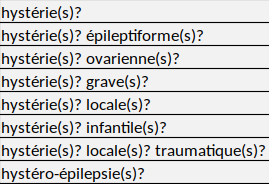
\includegraphics[width=30mm,scale=0.5]{pic/concepts-csv.png}
%\caption{Liste finale des concepts médicaux.}
%    \label{fig:my_label}
%\end{figure}
 \begin{figure}[!htb]
    \centering
    \begin{minipage}{.5\textwidth}
        \centering
        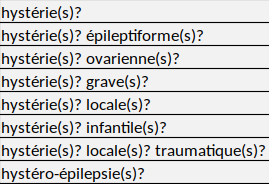
\includegraphics[width=0.6\linewidth, height=0.25\textheight]{pic/concepts-csv}
        \caption{Liste finale des concepts médicaux.}
        \label{fig:prob1_6_2}
    \end{minipage}%
    \begin{minipage}{.6\textwidth}
        \centering
   \begin{enumerate}
   \setcounter{enumi}{3}
   \item entre \texttt{<s>} et \texttt{,-(} (regex)
   \item sans termes génériques (\textit{os}, \textit{peau})
\item prise en compte des sg. / pl. (regex)
   \end{enumerate}
    \end{minipage}
\end{figure}
\end{frame}

\begin{frame}{Calcul de pertinence des concepts}
Trois mesures de pondération : \textsc{TF-IDF}, \textsc{BM25} et \textsc{BERT}.
    \footnotesize
\begin{table}[]
\begin{tabular}{|l|cccc|}
\hline
\multicolumn{1}{|c|}{\multirow{}{}{Terme}} & \multicolumn{4}{c|}{\cellcolor{gray!10!white}{ Corpus \og{}Autres\fg{}}}                              \\ \cline{2-5} 
\multicolumn{1}{|c|}{}                       & \multicolumn{1}{c}{{Fréquence}} & \multicolumn{1}{c}{{TF-IDF}} & \multicolumn{1}{c}{{BM25}}  & {BERT} \\ \hline
{Arthrite déformante} &
  \multicolumn{1}{|r|}{{24}} &
  \multicolumn{1}{|r|}{{0,02}} &
  \multicolumn{1}{|r|}{{0,50}} &
  {0,40} \\ \hline
{Ataxie locomotrice} &
  \multicolumn{1}{|r|}{{169}} &
  \multicolumn{1}{|r|}{{0,08}} &
  \multicolumn{1}{|r|}{{0,25}} &
  {0,39} \\ \hline
{Atrophie musculaire} &
  \multicolumn{1}{|r|}{{1465}} &
  \multicolumn{1}{|r|}{{0,43}} &
  \multicolumn{1}{|r|}{{0,15}} &
  {0,42} \\ \hline
{Atrophie progressive} &
  \multicolumn{1}{|r|}{{22}} &
  \multicolumn{1}{|r|}{{0,02}} &
  \multicolumn{1}{|r|}{{0,53}} &
  {0,39} \\ \hline
{Catalepsie} &
  \multicolumn{1}{|r|}{{975}} &
  \multicolumn{1}{|r|}{{0,28}} &
  \multicolumn{1}{|r|}{{0,15}} &
  {0,39} \\ \hline
{Épilepsie} &
  \multicolumn{1}{|r|}{{577}} &
  \multicolumn{1}{|r|}{{0,12}} &
  \multicolumn{1}{|r|}{{0,10}} &
  {0,41} \\ \hline
{Hystérie} &
  \multicolumn{1}{|r|}{{4934}} &
  \multicolumn{1}{|r|}{{0,45}} &
  \multicolumn{1}{|r|}{{0,05}} &
  {0,41} \\ \hline
{Langue} &
  \multicolumn{1}{|r|}{{3591}} &
  \multicolumn{1}{|r|}{{0,11}} &
  \multicolumn{1}{|r|}{{0,02}} &
  {0,41} \\ \hline
{Maladie de Parkinson} &
  \multicolumn{1}{|r|}{{130}} &
  \multicolumn{1}{|r|}{{0,09}} &
  \multicolumn{1}{|r|}{{0,35}} &
  {0,37} \\ \hline
{Paralysie bulbaire} &
  \multicolumn{1}{|r|}{{93}} &
  \multicolumn{1}{|r|}{{0,09}} &
  \multicolumn{1}{|r|}{{0,52}} &
  {0,40} \\ \hline
{Paralysie rhumatismale} &
  \multicolumn{1}{|r|}{{14}} &
  \multicolumn{1}{|r|}{{0,02}} &
  \multicolumn{1}{|r|}{{0,68}} &
  {\cellcolor{green!30!white}{\textcolor{purple}{\textbf{0,44}}}} \\ \hline
{Sclérose latérale} &
  \multicolumn{1}{|r|}{{127}} &
  \multicolumn{1}{|r|}{{0,09}} &
  \multicolumn{1}{|r|}{{0,37}} &
  {0,41} \\ \hline
{Sclérose en plaque disséminées} &
  \multicolumn{1}{|r|}{{12}} &
  \multicolumn{1}{|r|}{{0,02}} &
  \multicolumn{1}{|r|}{\cellcolor{green!30!white}{\textcolor{purple}{\textbf{0,83}}}} &
  {0,40} \\ \hline
{Somnambulisme} &
  \multicolumn{1}{|r|}{{3410}} &
  \multicolumn{1}{|r|}{\cellcolor{green!30!white}{\textcolor{purple}{\textbf{1}}}} &
  \multicolumn{1}{|r|}{{0,15}} &
  {0,43} \\ \hline
\end{tabular}
\caption{Pertinence des concepts sous forme des scores TF-IDF, BM25 et BERT, corpus \og{}Autres\fg{}.}
\end{table}
\end{frame} 

\begin{frame}{Intensification du discours
de Charcot dans le corpus \textrm{Autres}}
Le terme le plus impactant pour le réseau de Charcot selon \textsc{BM25} :\\
\textit{sclérose en plaque disséminées} ? (pertinence : 83\%)
\begin{figure}[!h]
    \centering
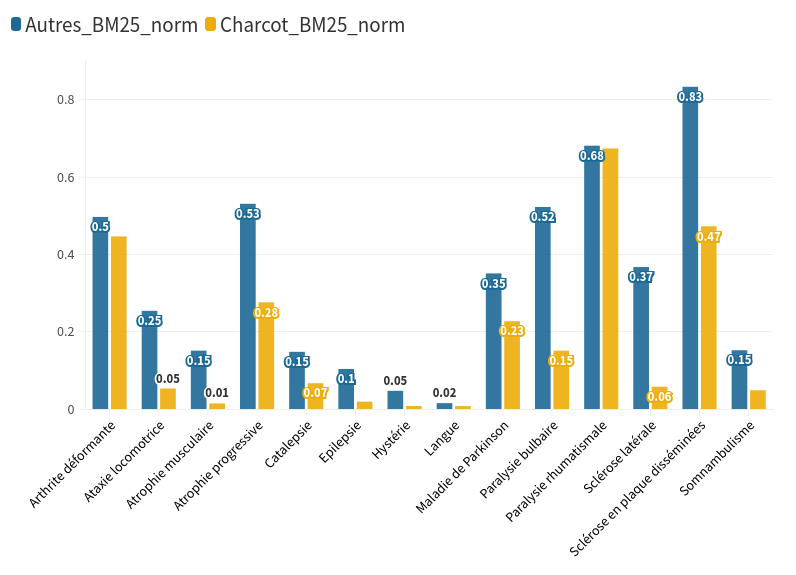
\includegraphics[width=80mm,scale=0.5]{pic/Charcot_Autres_250523.png}
    \caption{Pertinence des concepts dans les deux corpus (BM25).}
    \label{fig:my_label}
\end{figure}
\end{frame}

\begin{frame}{\textsc{BERT}}
\cite{vaswani2021}
    \begin{itemize}
        \item plongements lexicaux et des
mécanismes d’attention
        \item modèle \texttt{bert-base-multilingual-cased}
    \end{itemize}

\begin{table}[]
\begin{tabular}{|ll|ll|}
\hline
\multicolumn{2}{|c|}{\cellcolor[HTML]{EFEFEF}Corpus \og{}Charcot\fg{}} & \multicolumn{2}{c|}{\cellcolor[HTML]{EFEFEF}Corpus \og{}Autres\fg{}}     \\ \hline
\multicolumn{1}{|l|}{diplopie}                & 0,92 & \multicolumn{1}{l|}{préambule}       & 0,47      \\
\multicolumn{1}{|l|}{myélite partielle}       & 0,91 & \multicolumn{1}{l|}{délire}          & 0,47      \\
\multicolumn{1}{|l|}{état de mal épileptique} & 0,91 & \multicolumn{1}{l|}{miracle}         & 0,47      \\
\multicolumn{1}{|l|}{paralysie labio-glosso-laryngée} & 0,91 & \multicolumn{1}{l|}{cicatrices vicieuses} & 0,46 \\ \hline
\multicolumn{2}{|c|}{\cellcolor[HTML]{E1FFE1}\textsc{pathologies}}     & \multicolumn{2}{c|}{\cellcolor[HTML]{FFDFDD}\textsc{notions abstraites}} \\ \hline 
\end{tabular}
\end{table}
\end{frame}
\section[Approche non supervisée]{Approche non supervisée}
%\begin{frame}{Extraction des phrases-clés}
%\og{}\textcolor{deepblue}{Phrases-clés}\fg{}, angl. \textit{keyphrases}
%\begin{itemize}
%\item séquences de plusieurs mots (ex. \textit{sclérose latérale amyotrophique})
%\item reflètent plus précisément le contexte sémantique du texte \\\small{$\neq$ mots-clés, angl. \textit{keywords} : unigrammes de mot (ex. \textit{sclérose})}
%\end{itemize}
%\bigskip
%%\centering
%%Extraction de \og{}phrases-clés\fg{} (angl. \textit{keyphrases})
%%\\~\\
%%\begin{block}{Extraction de phrases-clés}
%%\justifying
%%Processus de \underline{sélection} automatique d'un petit ensemble de phrases les plus pertinentes à partir d'un texte donné \citep{schopf2022}.
%%\end{block}
%%\begin{block}{Prédiction de phrases-clés}
%%\justifying
%%Processus de \underline{génération} des phrases-clés qui résument parfaitement un document donné \citep{xie2023}.
%\begin{columns}[t,onlytextwidth]
%\column{.45\textwidth}
%\textcolor{violet}{Extraction}
%\justifying
%
%Processus de \underline{sélection} automatique d'un petit ensemble de phrases les plus pertinentes à partir d'un texte donné.
%\vspace{-0.2cm}
%\begin{flushright}
%\small{\citep{schopf2022}}
%\end{flushright} 
%\column{.45\textwidth}
%\textcolor{violet}{Prédiction}
%\justifying
%
%Processus de \underline{génération} des phrases-clés qui résument parfaitement un document donné.
%\vspace{0.3cm}
%\begin{flushright}
%\small{\citep{xie2023}}
%\end{flushright}
%\end{columns}%Extraction de phrases-clés
%%
%%Processus de \underline{sélection} automatique d'un petit ensemble de phrases les plus pertinentes à partir d'un texte donné \citep{schopf2022}.
%%
%%\begin{block}{Prédiction de phrases-clés}
%%\justifying
%%Processus de \underline{génération} des phrases-clés qui résument parfaitement un document donné \citep{xie2023}.
%%\end{block} 
%\end{frame}

\begin{frame}{Extraction des phrases-clés : méthode \texttt{keybert}}
\begin{enumerate}
\small
\item entrée : un document
\item tokénisation du document en phrases-clés candidates (PCC)
\item génération des plongements du doc. et des PCC par un modèle de langage
\item calcul de la similarité cosinus entre le document et les PC
\end{enumerate}
\begin{figure}
    \centering
    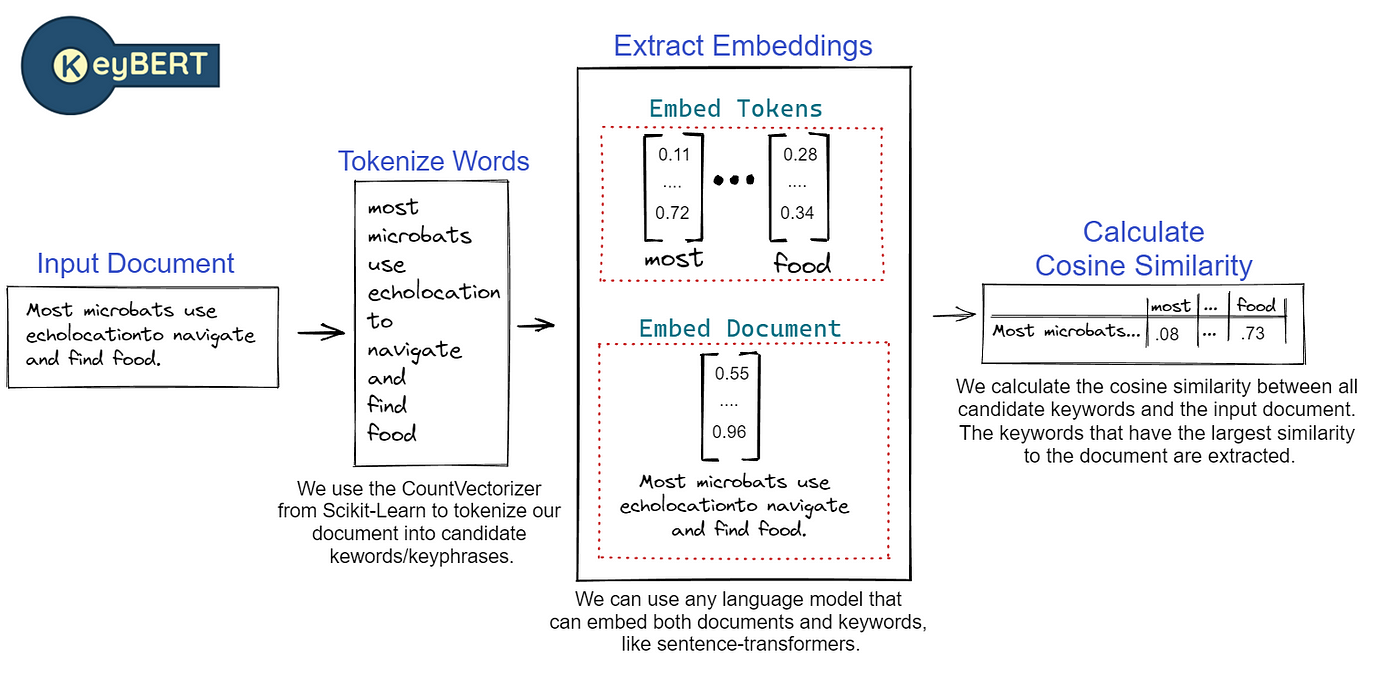
\includegraphics[width=80mm,scale=0.5]{pic/keybert.png}
    \caption{\textit{Pipeline} de la librairie \texttt{keybert} \citep{grootendorst2020keybert}.}
    \label{fig:enter-label}
\end{figure}
\end{frame}

\begin{frame}{Limitations de \texttt{keybert}}
\danger{} manque de diversification des résultats + (non-)grammaticalité\\
    \begin{figure}[!ht]
        \centering
        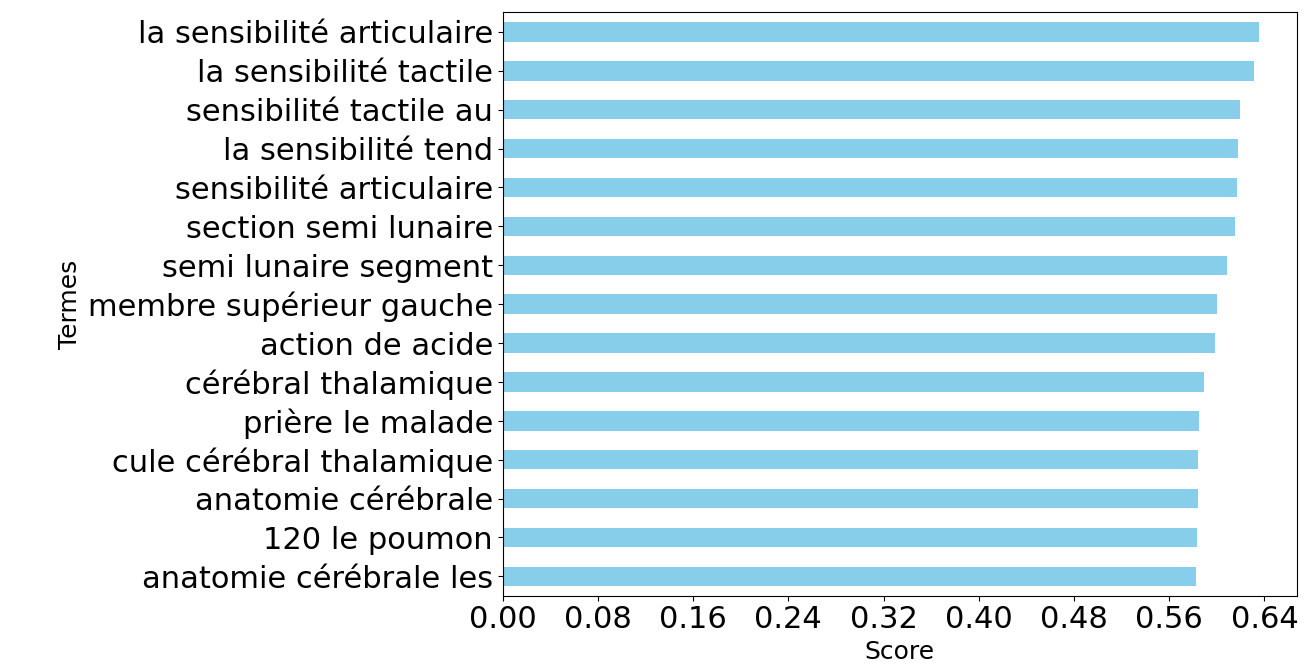
\includegraphics[width=110mm,scale=0.5]{pic/termes_keybert_autres.png}
        \caption{Répartition des 15 termes les plus pertinents dans le corpus \og{}Autres\fg{} selon \texttt{keybert}.}
        \label{fig:enter-label}
    \end{figure}
\end{frame}

\begin{frame}{Phrases-clés \textit{hapax} partagés dans les deux corpus selon \texttt{keybert}}
Les seuls termes partagés avec le corpus Charcot : 
%\begin{itemize}
%\item articulations de [\textit{sic}] épaule
%\item paralysie faciale périphérique
%\end{itemize}
    \begin{figure}[!ht]
        \centering
        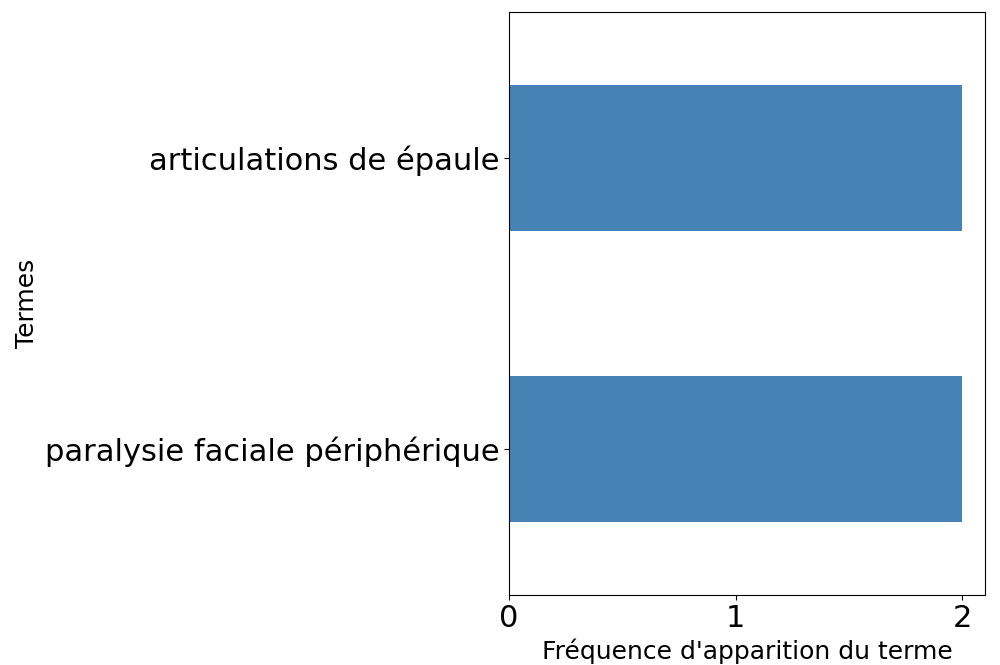
\includegraphics[width=90mm,scale=0.5]{pic/termes_partages_keybert.png}
        \caption{Répartition des termes les plus pertinents dans les deux corpus selon \texttt{keybert}.}
        \label{fig:enter-label}
    \end{figure}
\end{frame}
\begin{frame}{Extraction des phrases-clés : méthode \textit{PatternRank}\\
\quad \quad \quad\ \quad \quad \quad \quad \quad \quad \quad \ \ \ \ \ \small{Librairie \texttt{keyphrase-vectorizers}}}
%\begin{itemize}
%\item extraction des phrases-clés non-supervisée
%\item exploite des modèles de langues pré-entraînés + parties du discours
%\end{itemize}
\begin{enumerate}
\small
\item entrée : un seul document texte tokenisé
\item étiquetage des tokens avec les balises du partie du discours (POS)
\item sélection des tokens selon le motif POS $\rightarrow$ phrases-clés candidates (PCC)
\item génération des plongements du doc. et des PCC par un modèle de langue
\item calcul des similarités cosinus entre ces deux types de plongements +  \\classement des PCC par ordre décroissant
\item extraction des \textit{N} PC les plus représentatives
\end{enumerate}
\begin{figure}
    \centering
    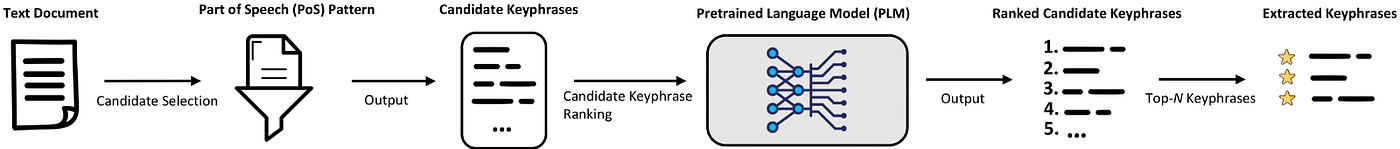
\includegraphics[width=110mm,scale=0.5]{pic/patternrank_workflow.png}
    \caption{\textit{Workflow} de la méthode \textit{PatternRank} \citep{schopf2022}.}
    \label{fig:enter-label}
\end{figure}
\notecite{schopf2022}
\end{frame}

%\begin{frame}{Termes partagés extraits avec \texttt{keyphrase-vectorizers}}
%    \begin{figure}[!ht]
%        \centering
%        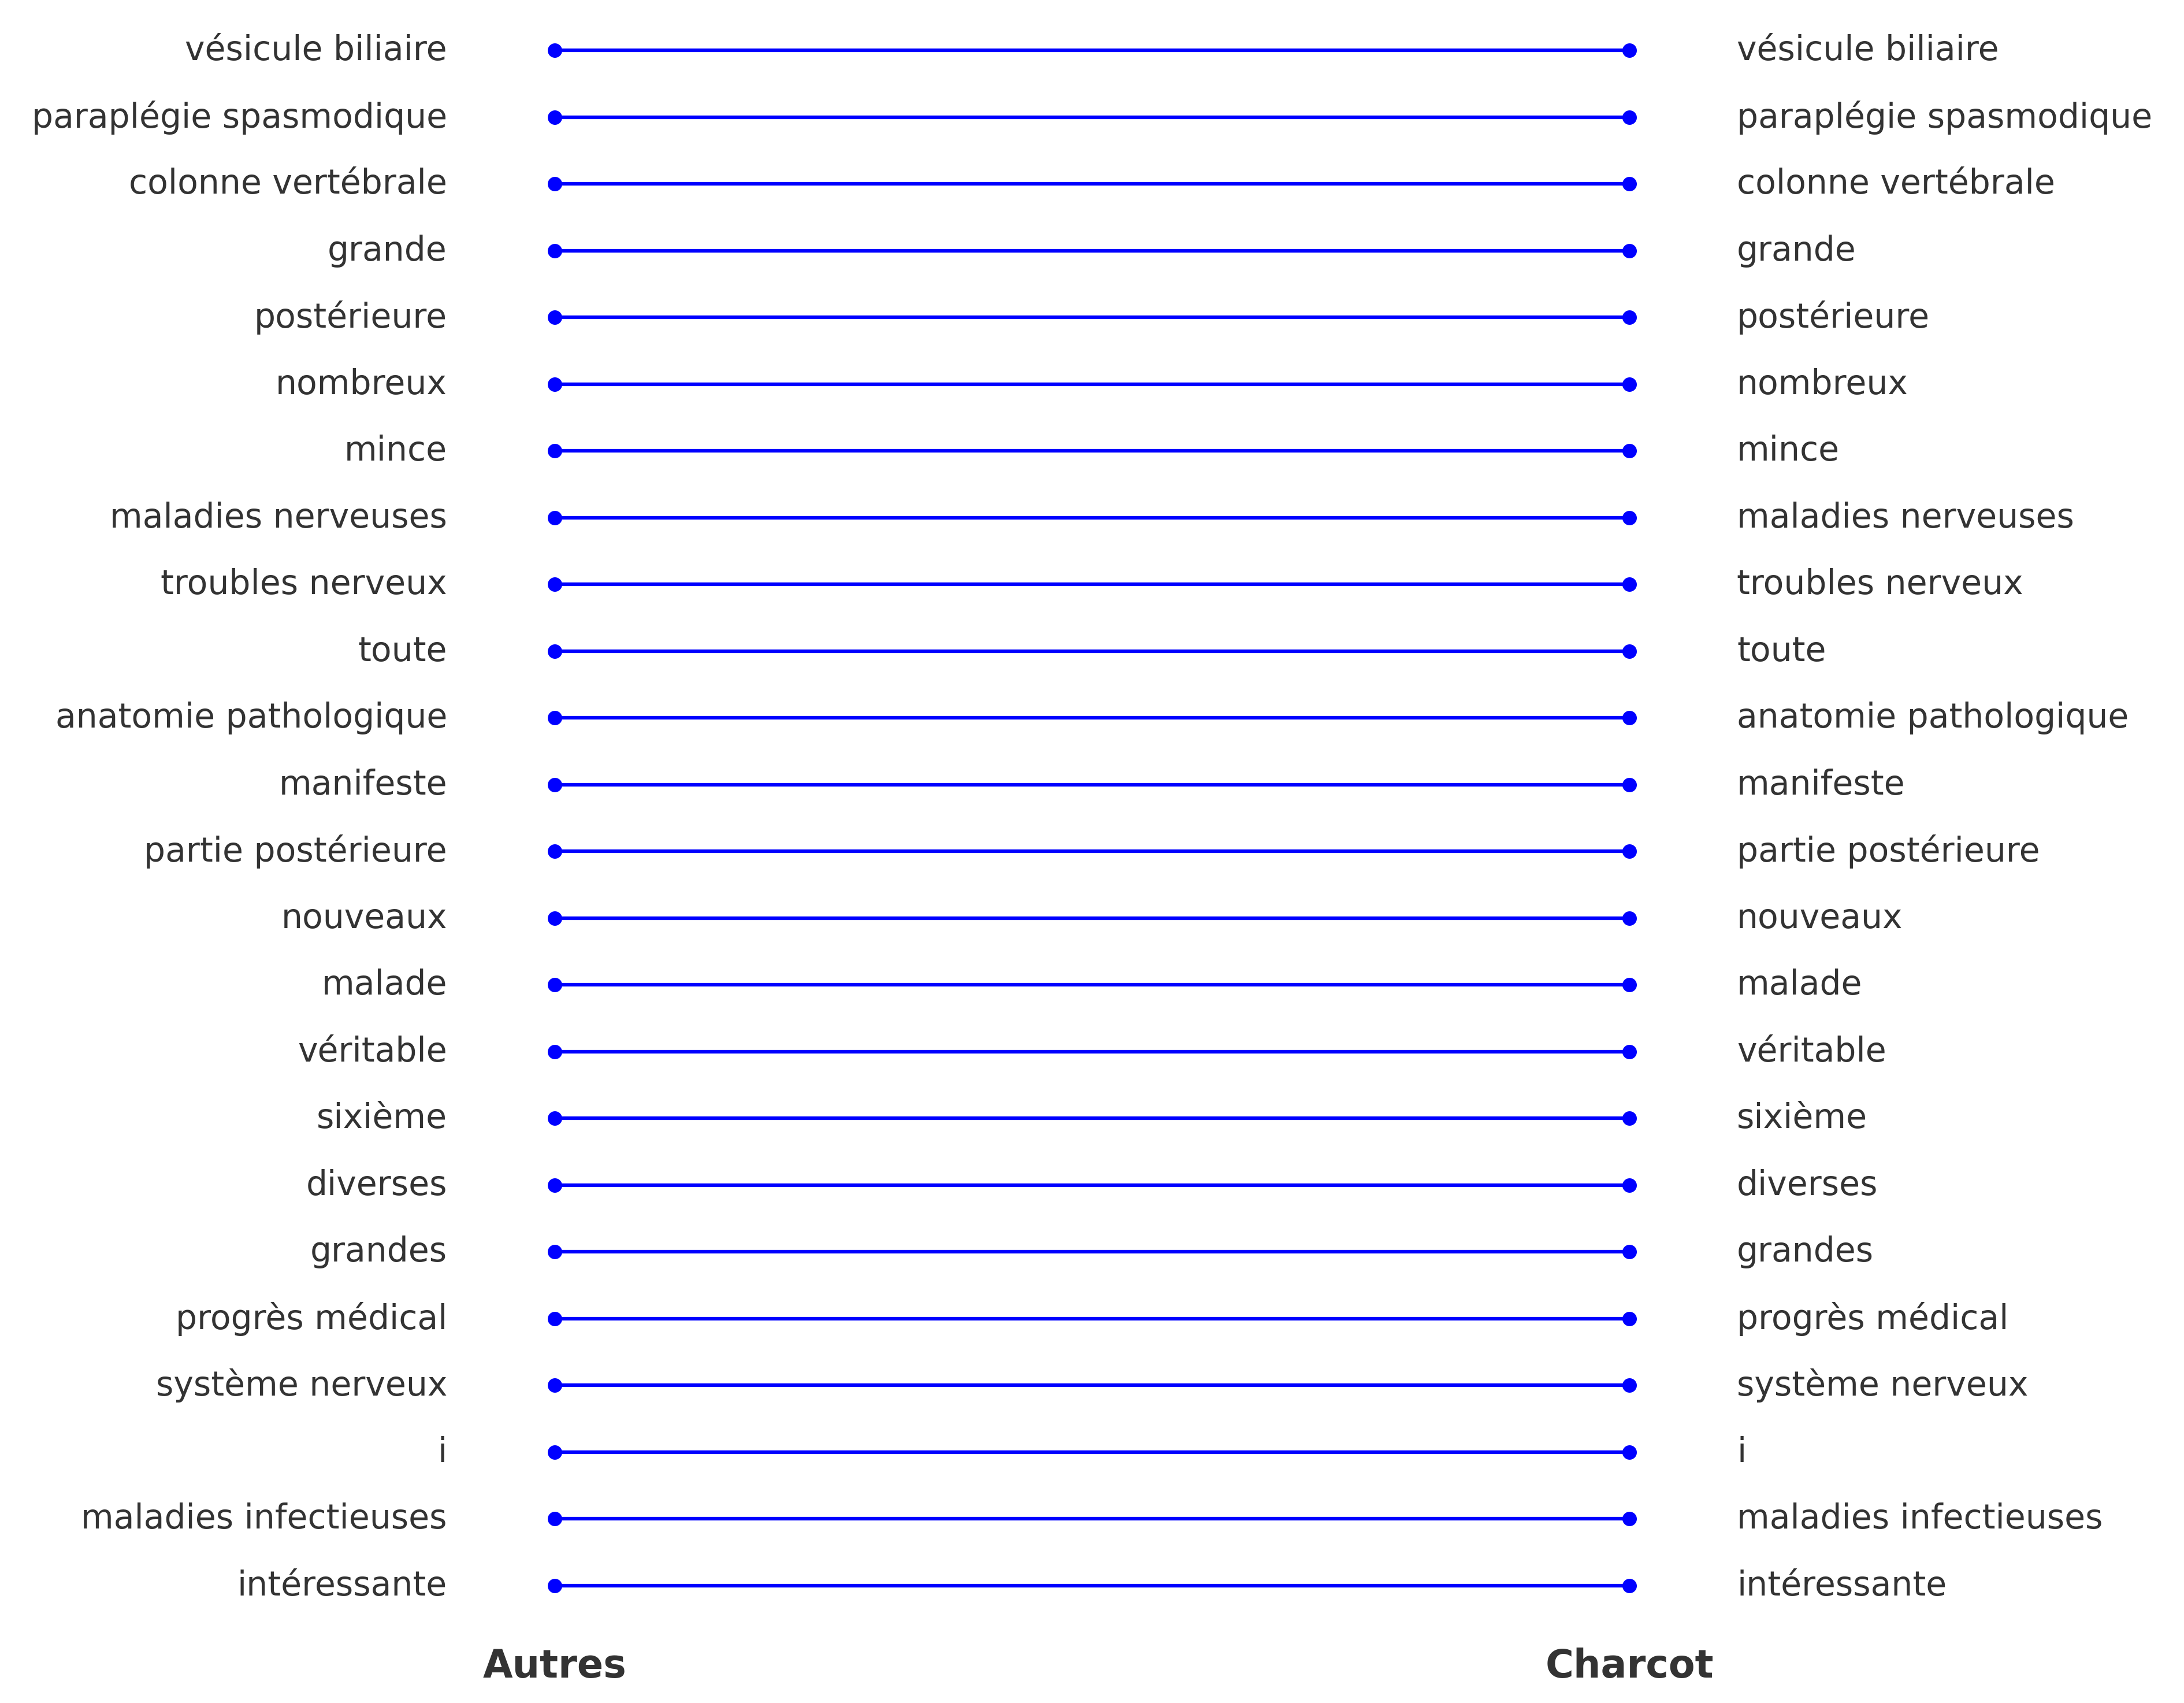
\includegraphics[width=85mm,scale=0.5]{pic/visualisation_termes_dupliques.png}
%        \caption{Les termes communs aux deux corpus selon \texttt{keyphrase-vectorizers}.}
%        \label{fig:enter-label}
%    \end{figure}
%\end{frame}

%\begin{frame}{Termes partagés | \texttt{keyphrase-vectorizers}}
%    \begin{figure}[!ht]
%        \centering
%        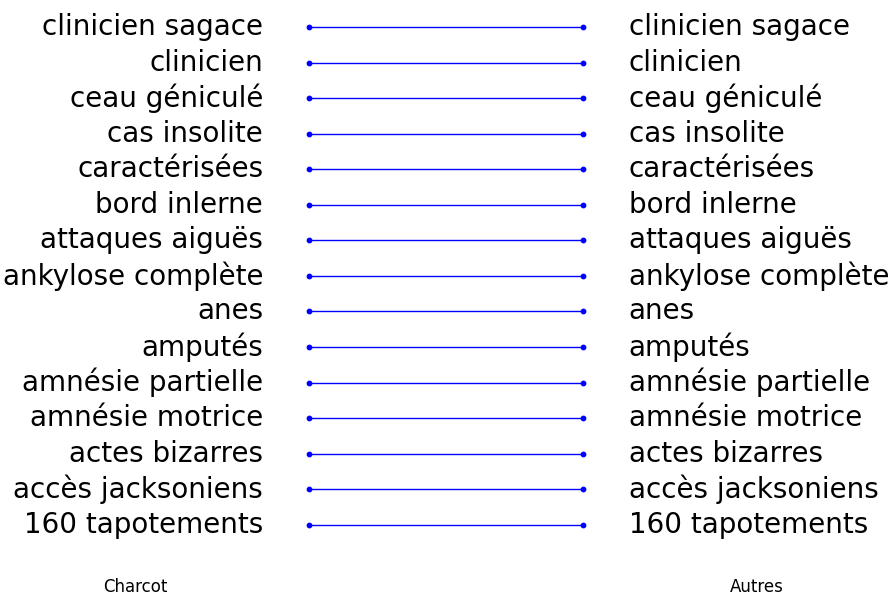
\includegraphics[width=100mm,scale=0.5]{pic/termes_partages_liens.png}
%        \caption{Les termes communs (fréq. = 1) aux deux corpus selon \texttt{keyphrase-vectorizers}.}
%        \label{fig:enter-label}
%    \end{figure}
%\end{frame}

\begin{frame}{Les termes partagés les plus fréquents | \texttt{keyphrase-vectorizers}}
    \begin{figure}[!ht]
        \centering
        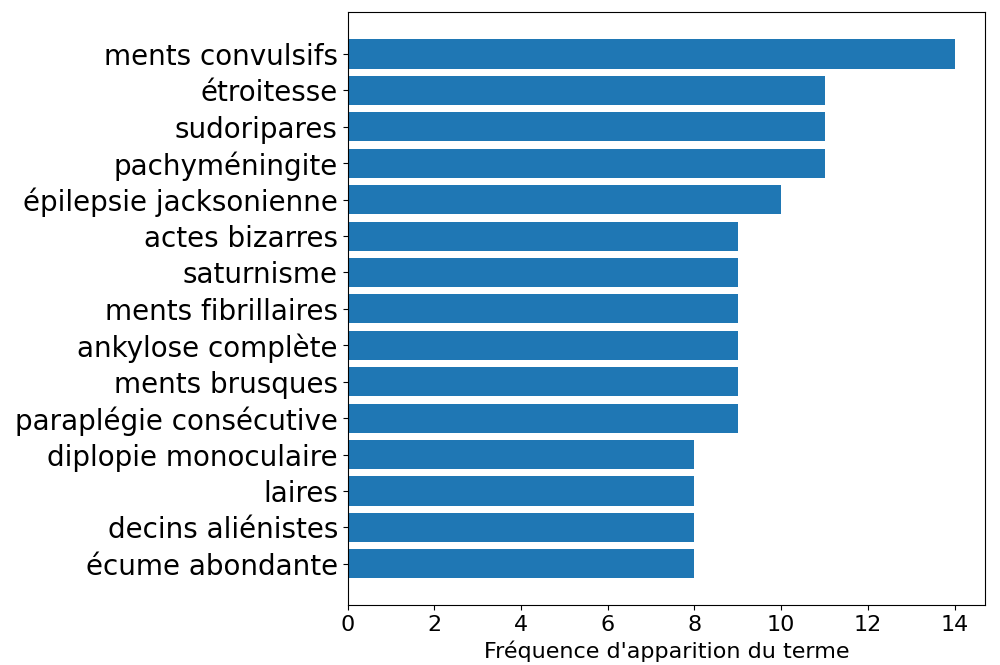
\includegraphics[width=100mm,scale=0.5]{pic/termes_partages.png}
        \caption{Les 15 termes les plus fréquents dans les deux corpus selon \texttt{keyphrase-vectorizers}.}
        \label{fig:enter-label}
    \end{figure}
\end{frame}

%\begin{frame}{Accès à la plateforme technologique \textsc{MeSU}}
%\begin{itemize}
%\item expériences réalisées sur la plateforme \href{https://sacado.sorbonne-universite.fr/}{\textsc{MeSU}} de Sorbonne Université
%\end{itemize}
%\bigskip
%
%Les données et les scripts utilisés dans le cadre de cette étude sont disponibles sur le \href{https://github.com/ljpetkovic/JE\_IA\_HN\_030524}{dépôt GitHub}.
%\end{frame}
\section[Conclusion]{Conclusion et recherches futures}
\begin{frame}{Conclusion et recherches futures}
Contributions :
\begin{itemize}
\item étendue de l'impact de Charcot sur la neurologie
\item étude numérique de son héritage scientifique
\end{itemize}
\bigskip
Prochaines étapes :
\begin{enumerate}
\item diversification des phrases-clés extraites par \texttt{keybert}
\item définir les notions des \textsc{circulations numériques} et du \textsc{concept} du point de vue du \textsc{TAL} / linguistique
\item évaluation des phrases-clés extraites (semi-)automatique +  \\
retour d'un spécialiste de Charcot 
\item contexte des réemplois textuels (affirmation, contestation $\dots$)
\end{enumerate} 
\end{frame}


\begin{frame}{Remerciements}
Un grand merci à :
\begin{itemize}
\item Valentina Fedchenko\\
{\small \textcolor{gray}{ingénieure de recherche, équipe-projet \textsc{ObTIC}}}
\item Motasem Alrahabi\\
{\small \textcolor{gray}{ingénieur de recherche, équipe-projet \textsc{ObTIC}}}
\item Glenn Roe\\
{\small \textcolor{gray}{professeur des univerités, équipe-projet \textsc{ObTIC}}}
\item Simon Gabay\\
{\small \textcolor{gray}{maître-assistant, Chaire des humanités numériques, univ. de Genève}}
\item unité de service \textsc{SACADO}\\
{\small \textcolor{gray}{hébergeur de la plateforme \textsc{MeSU} de Sorbonne Université, sur laquelle les expériences ont été realisées}}
\end{itemize}
\end{frame}

\begin{frame}{Dépôts GitHub}
\begin{center}
Les données et les scripts utilisés dans le cadre de cette étude sont disponibles dans les dépôts GitHub suivants :
\begin{itemize}
\small
\item \href{https://github.com/ljpetkovic/JE\_IA\_HN\_030524}{Mesurer l’influence de Charcot sur ses contemporains à l’aide de l’extraction de phrases-clés}
\item \href{https://github.com/ljpetkovic/Charcot\_circulations}{\textit{Tracking the circulation of Jean-Martin Charcot’s medical discourse: first observations}}.
\end{itemize} 
\end{center}
\end{frame}
%\section[État de l'art]{État de l'art}
%\begin{frame}{Extraction des mots-clés : état de l'art}
\begin{figure}
    \centering
    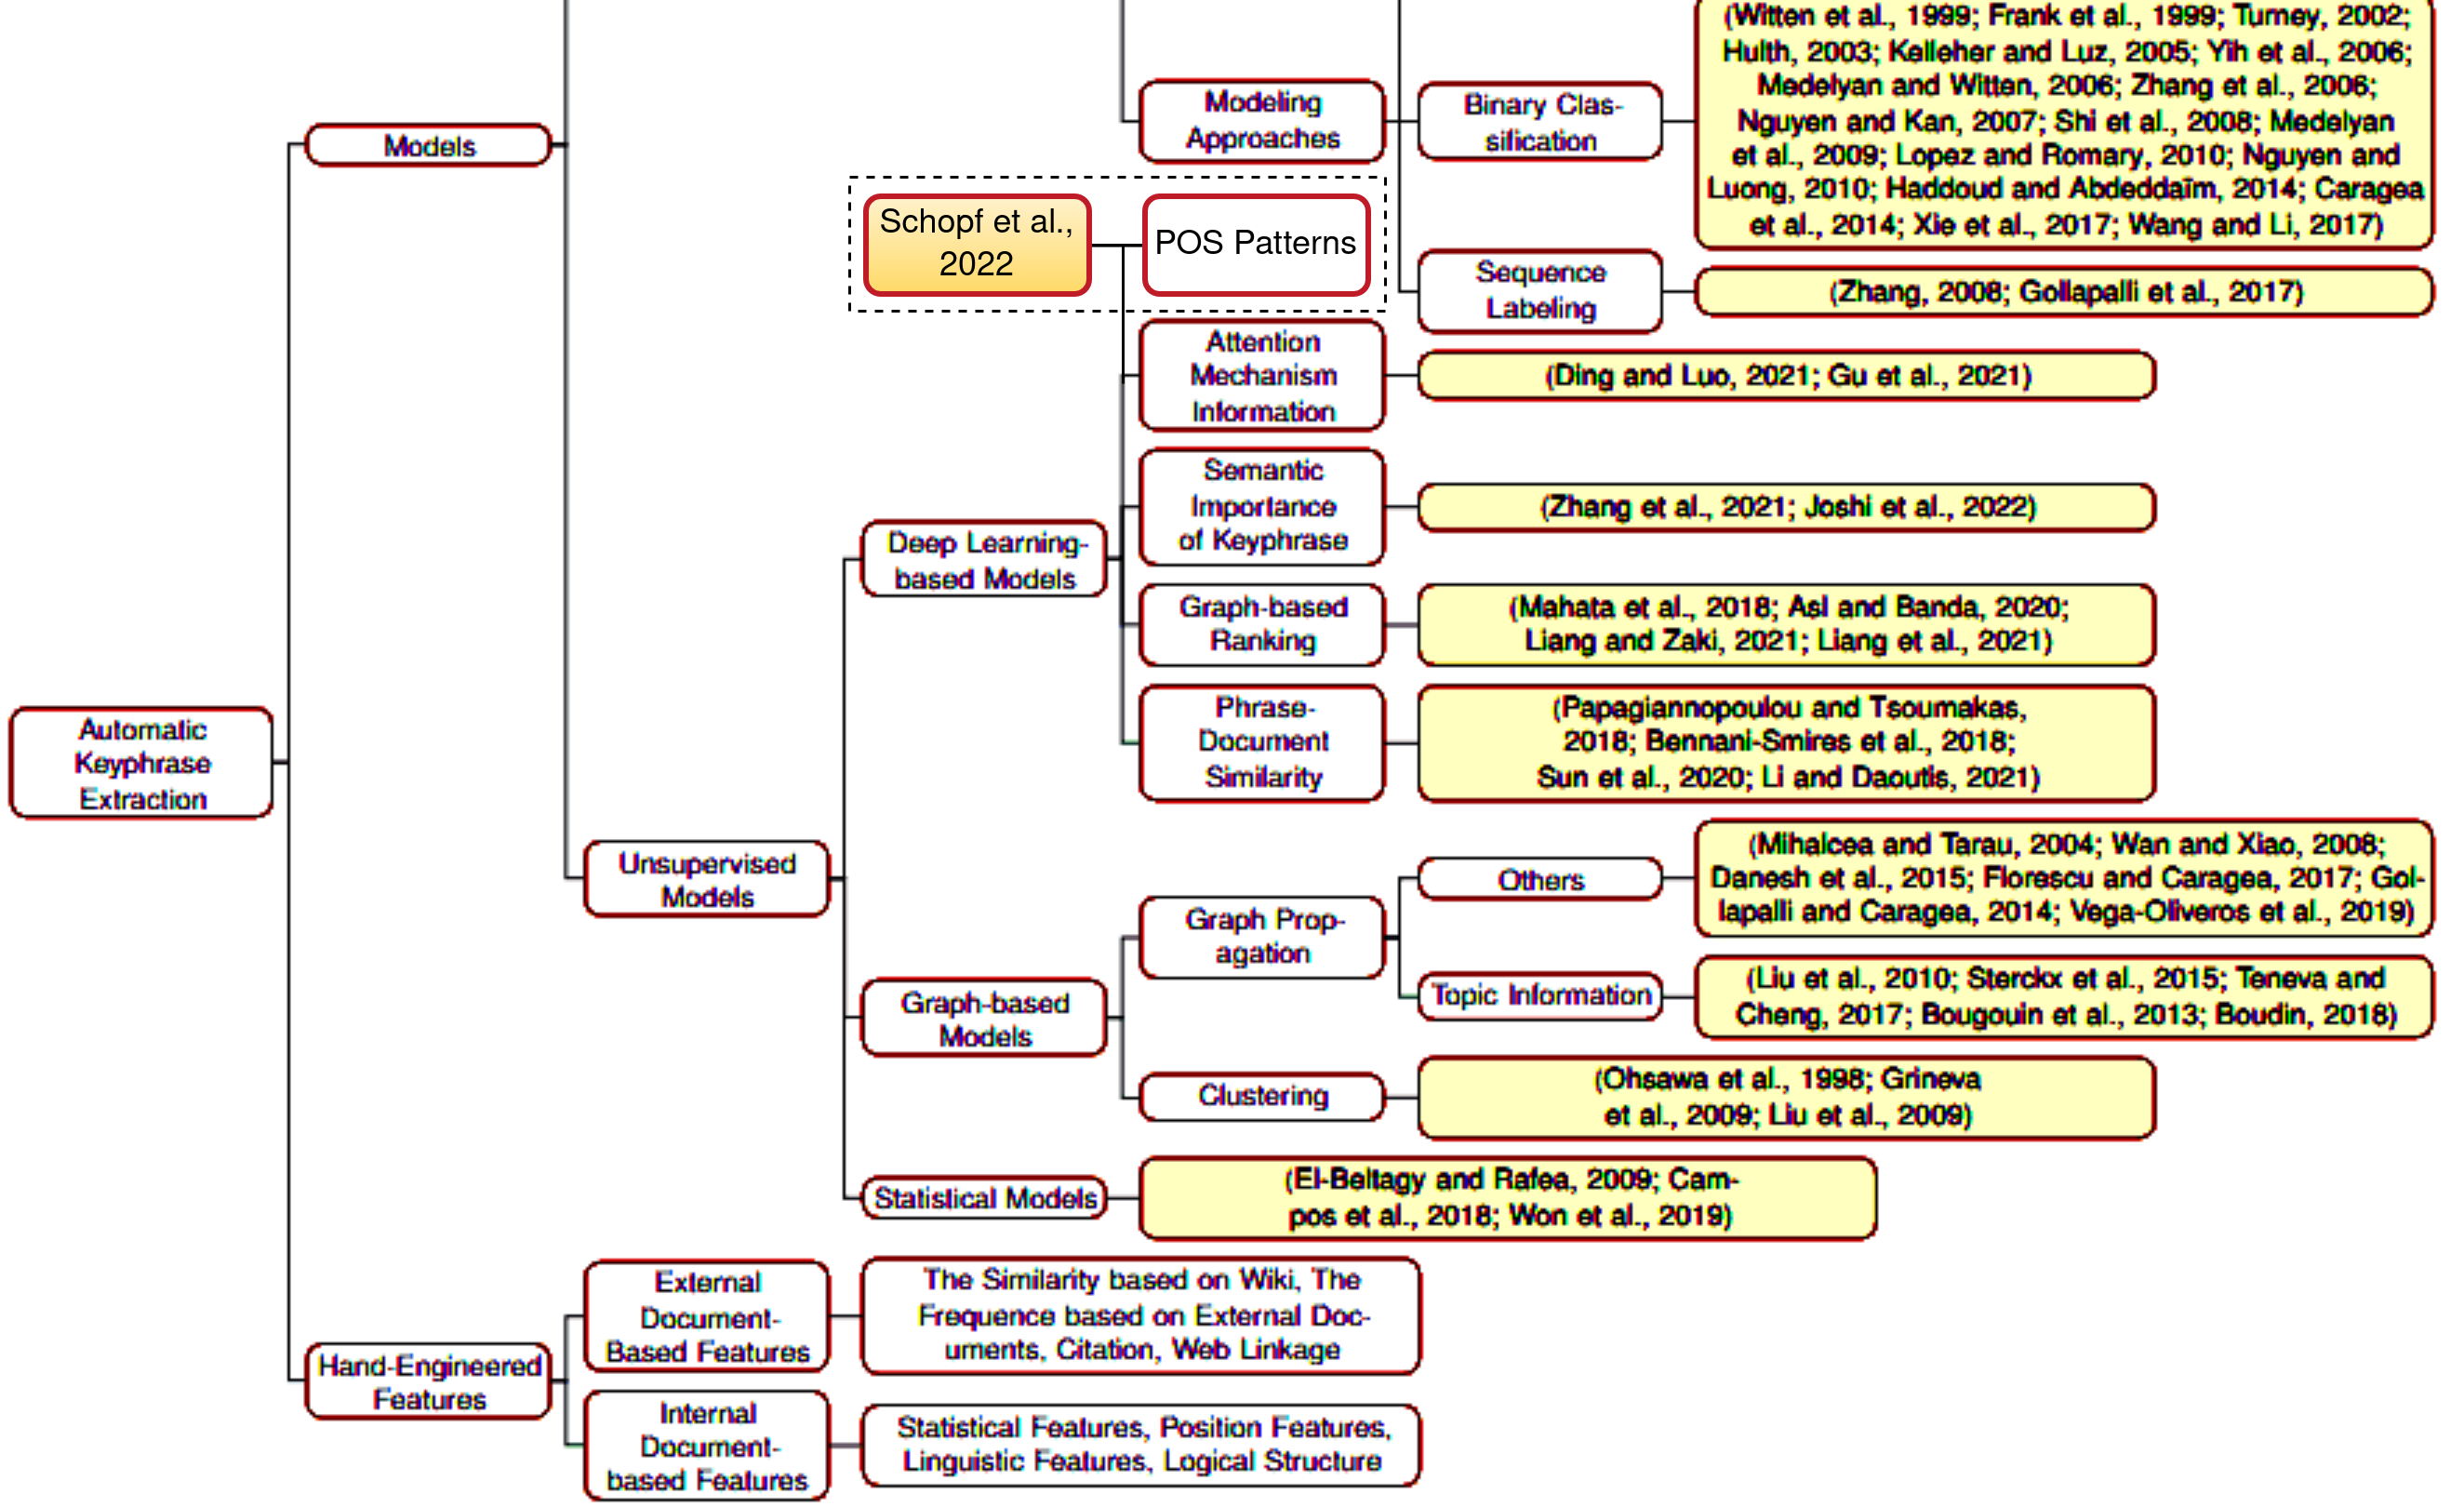
\includegraphics[width=105mm,scale=0.5]{pic/sota_adapte.png}
    \caption{Extrait de l'état de l'art sur l'extraction des mots-clés, adapté de \citet{xie2023}\footnote{Figure retouchée pour raison de lisibilité.}.}
    \label{fig:enter-label}
\end{figure}
\end{frame}
%\section[\textit{PatternRank}]{\textit{PatternRank}}
%\begin{frame}{\textit{PatternRank}}
\begin{figure}
    \centering
    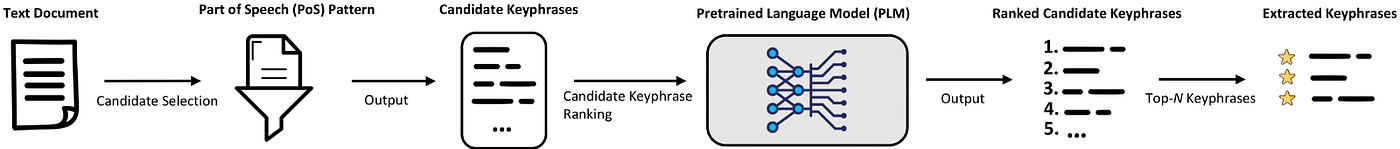
\includegraphics[width=50mm,scale=0.5]{pic/patternrank_workflow.png}
    \caption{\textit{Workflow} de la méthode \textit{PatternRank}.}
    \label{fig:enter-label}
\end{figure}
\citep{schopf2022}
\end{frame}



% \appendix

\begin{frame}[allowframebreaks]{Références}
\printbibliography

\end{frame}

\end{document}